\section{Related work}

\subsection{Model learning}

\subsubsection{World Models}

In World Models\cite{Algo.WorldModels} paper, the authors explore the idea of using large and highly expressive neural networks, that can learn rich spatial and temporal representation of data, and applying them to reinforcement learning. The RL algorithm is often bottlenecked by the credit assignment problem, which makes it hard for traditional RL algorithms to learn millions of weights of a large model. To accomplish their goal, they decompose the problem of an agent training into two stages: they first train a generative neural network to learn a model of the agent's world in an unsupervised manner. Thereafter, by using a compressed spatial and temporal representation of the environment extracted from the world model as inputs to the agent, they train a linear model to learn to perform a task in the environment. The small linear model lets the training algorithm focus on the credit assignment problem on a small search space, while not scarifying capacity and expressiveness via the larger world model.

Their solution consists of three components: Vision (V) for encoding the spatial information, Memory (M) for encoding the temporal information and Controller (C) which represents the agent's policy. Fig.~\ref{Fig.WorldModels} depicts a flow diagram of the agent's model.

\begin{figure}[H]
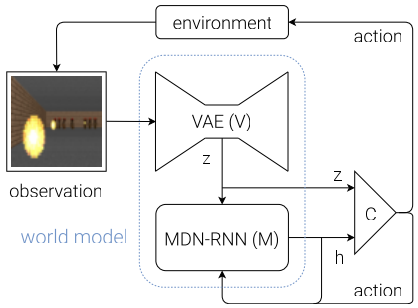
\includegraphics[width=0.7\textwidth,keepaspectratio]{figures/WorldModels.png}
\caption[Flow diagram of the World Models agent's model]{Flow diagram of the agent's model\protect\cite{Algo.WorldModels}. The raw observation is first processed by V at each time step $t$ to produce $z_t$. The input into C is this latent vector $z_t$ concatenated with M’s hidden state $h_t$ at each time step. C will then output an action vector $a_t$ and will affect the environment. M will then take the current $z_t$ and action $a_t$ as an input to update its own hidden state to produce $h_{t+1}$ to be used at time $t + 1$.}
\label{Fig.WorldModels}
\end{figure}

The environment provides the agent with high dimensional visual observation at each time step. The essential task of the Vision model is to encode this high dimensional observation into a low dimensional latent state. To do this, Vision is implemented as Variational Autoencoder\cite{Algo.VAE}. It is trained in an unsupervised manner on randomly generated experience from the environment.

Since many complex environment are partially observable, the visual observation at each time step, and hence the latent state, doesn't include full information about the current situation in the environment. To acquire full knowledge, the agent needs to encode what happens over time. This is the role of the Memory model. It is implemented as Recurrent Neural Network\cite{Algo.LSTM} (RNN) and trained on the same data as Vision to predict the future latent state that Vision is expected to produce. Because many environments are stochastic in nature, the RNN is trained to output a probability density of the next latent state approximated as a mixture of Gaussian distribution - in literature, this approach is known as Mixture Density Network combined with a RNN (MDN-RNN)\cite{Algo.MDNRNN}. More specifically, the RNN will model $P(z_{t+1}|a_t,z_t,h_t)$, where $z_{t+1}$ is the output next latent state, $a_t$ is the action taken at time $t$, $z_t$ is the latent state of the current time step $t$ and $h_t$ is the hidden state of the RNN that encodes past information made available to the agent from the beginning of the episode until the time step $t$.

The Controller model represents the agent's policy. It is responsible for determining course of actions to take in order to solve a given task. Controller is a simple linear model that maps the concatenated latent state $z_t$ and hidden state $h_t$ at the time step $t$ directly to the action $a_t$ at that time step: $a_t = W[z_t h_t] + b$, where $W$ and $b$ are the weight matrix and bias vector of that model.
The authors deliberately made Controller as simple as possible, and trained it separately from Vision and Memory, so that most of the agent's complexity resides in the world model (V and M). The latter can take the advantage of current advances in deep learning that provide tools to train large models efficiently when well-behaved and differentiable loss function can be defined.
Shift in the agent's complexity towards the world model allows the Controller model to stay small and focus its training on tackling the credit assignment problem in challenging RL tasks. It is trained using evolution strategy, which is rather an unconventional choice that only currently have been considered as a viable alternative to popular RL techniques\cite{Algo.ESRL}.

Their solution was able to solve an OpenAI Gym's CarRacing environment, which is the continuous-control, top-down racing task. It is the first known solution to achieve the score required to solve this task. In the process, the Memory model have learned to simulate the original environment. The authors show that the learned policy can function inside of the imagined environment of CarRacing, that is simulated by Memory.
In the second experiment, they show that the agent is able to learn from imagined experience, produced by its Memory, and successfully transfer this policy back to the actual environment of VizDoom (see fig.~\ref{Fig.VizDoom}). This result indicates that the world model is able to model complex environments from visual observations and it can be used for planning. Therefore, it may prove useful for the topic of this thesis. \editnote{Should we expand on that in here? Or rather place for that is in ``Planning with learned model'' chapter where I describe design of my solution?}

\begin{figure}[H]
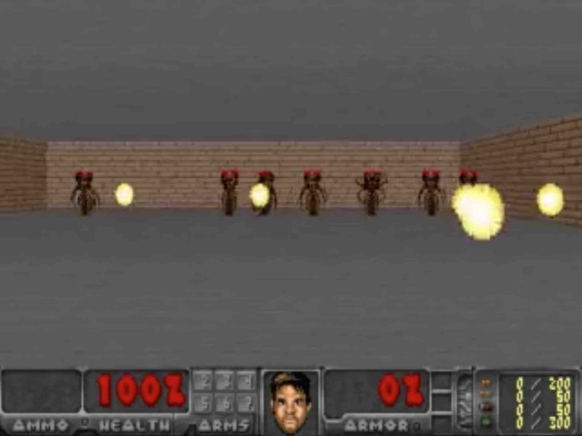
\includegraphics[width=0.7\textwidth,keepaspectratio]{figures/VizDoom.png}
\caption[VizDoom]{VizDoom: the agent must learn to avoid fireballs shot by monsters from the other side of the room with the sole intent of killing the agent\protect\cite{Algo.WorldModels}.}
\label{Fig.VizDoom}
\end{figure}
